\documentclass[10pt]{article}
\usepackage[utf8]{inputenc}
\usepackage[T1]{fontenc}
\usepackage{graphicx}
\usepackage{appendix}
\usepackage[french]{babel}
\usepackage{fancyhdr}
\usepackage{geometry}
\geometry{hmargin=3cm,vmargin=3.5cm}
\usepackage{enumitem}
\usepackage{listings}
\usepackage{subcaption}
\usepackage{amsmath}
\usepackage{fixltx2e}
\usepackage{algorithm}
\usepackage{algpseudocode}
\graphicspath{{./img/}}
\lstset{ %
  backgroundcolor=\color{white},   % choose the background color; you must add \usepackage{color} or \usepackage{xcolor}
  basicstyle=\small,               % the size of the fonts that are used for the code
  breakatwhitespace=false,         % sets if automatic breaks should only happen at whitespace
  breaklines=true,                 % sets automatic line breaking
  captionpos=b,                    % sets the caption-position to bottom
  commentstyle=\color{blue},      % comment style
%  escapeinside={\%*}{*)},          % if you want to add LaTeX within your code
  extendedchars=true,              % lets you use non-ASCII characters; for 8-bits encodings only, does not work with UTF-8
  frame=single,                    % adds a frame around the code
  keepspaces=true,                 % keeps spaces in text, useful for keeping indentation of code (possibly needs columns=flexible)
%  keywordstyle=\color{blue},       % keyword style
  language=C,                    % the language of the code
  numbers=left,                    % where to put the line-numbers; possible values are (none, left, right)
  numbersep=5pt,                   % how far the line-numbers are from the code
  numberstyle=\tiny\color{black},  % the style that is used for the line-numbers
  rulecolor=\color{black},         % if not set, the frame-color may be changed on line-breaks within not-black text (e.g. comments (green here))
  showspaces=false,                % show spaces everywhere adding particular underscores; it overrides 'showstringspaces'
  showstringspaces=false,          % underline spaces within strings only
  showtabs=false,                  % show tabs within strings adding particular underscores
  stepnumber=1,                    % the step between two line-numbers. If it's 1, each line will be numbered
  tabsize=2,                       % sets default tabsize to 2 spaces
}
\usepackage{stmaryrd}
\usepackage{hyperref}
\hypersetup{colorlinks=true}

\pagestyle{fancy}

\renewcommand{\sectionmark}[1]{ \markright{#1}{} }

\MakeRobust{\For}
\MakeRobust{\Call}

\lhead{}
\rhead{}
\lfoot{ENSEIRB-MATMECA}
\rfoot{PRCD}
\renewcommand{\headrulewidth}{0.pt}
\renewcommand{\footrulewidth}{0.4pt}


\title{TDP5}
\author{Alexandre Honorat}
\date{\today}

\begin{document}
%\tableofcontents
%\newpage

\thispagestyle{empty}


%\begin{center}
%
\includegraphics{enseirb_inp.png}
%\end{center}
%
%\vspace{\stretch{1}}
\hrule
\begin{flushleft}
\Huge{\textbf{TDP4 - Utilisation de MPI}}\\
\textit{Lancer de Rayons}
\end{flushleft}
\begin{flushright}
\huge\textbf{Rapport}\\
\end{flushright}
\hrule

\vspace{80pt}
\noindent\textbf{Élèves :}
\emph{Alexandre Honorat}, \emph{Elouan Keryell-Even}\\
\\
\noindent\textbf{Responsable :}
\emph{Astrid Casadei}\\


\vspace{60pt}
\normalsize
\begin{center}
  Troisième année, filière informatique, option PRCD\\
  Date : \today\\
  Enseirb-Matmeca
\end{center}
\vspace{50pt}

%% -*- eval: (flyspell-mode 1); -*-

\chapter{Introduction}
%\addcontentsline{toc}{chapter}{Introduction}

Un des aspects de la recherche informatique consiste à améliorer des programmes afin de rendre leur temps d'exécution plus rapide, il s'agit du \emph{calcul haute performance} (ou HPC, pour High Performance Computing). 
%Les performances -- en matière de temps d'exécution -- sont primordiales par exemple pour les codes de simulation numérique dédiés à la météorologie qui calculent les prévisions du lendemain, où bien entendu la simulation doit donc s'être terminée en moins d'une nuit. 
Dans ce cadre le stage a porté sur la génération automatique de certains de ces programmes améliorés. 
Les sections suivantes présentent brièvement quelques rappels sur les problématiques HPC, ainsi que l'objectif du stage : l'adaptation automatique d'une certaine catégorie de problèmes au matériel prévu pour le HPC. Le chapitre $2$ précise plus particulièrement ces problématiques et l'objectif tandis que le chapitre $3$ se concentre sur le travail réalisé. Le chapitre $4$ en propose une évaluation et est suivi par la conclusion. 


\section{Parallélisation de programmes}

Diverses techniques existent pour améliorer les performances d'un programme et plus particulièrement de son temps d'exécution. Deux aspects peuvent entrer en compte : les algorithmes utilisés dans le programme ainsi que le matériel qui l'exécute. Le facteur limitant à améliorer en priorité est alors le matériel, car il influe sur la nature des algorithmes pouvant être utilisés.

La solution la plus simple pour améliorer les performances consisterait à se baser uniquement sur la loi de Moore, c'est-à-dire sur le fait que les capacités du matériel sur lequel le programme est exécuté sont doublées tous les ans. Or cette loi exponentielle n'est maintenant plus valable puisque la fréquence d'horloge des processeurs modernes stagne depuis quelques années à une valeur proche de $3$ GHz. 
%C'est cette fréquence d'horloge qui impose au matériel (si celui-ci est constitué de cet unique processeur) le nombre d'opérations qu'il va pouvoir effectuer en une seconde. Puisque la fréquence n'augmente plus, le nombre d'opérations par seconde pour ce type de matériel ne peut plus augmenter non plus, aucun gain de rapidité d'exécution n'est alors possible.

%La première solution s'appuyait ainsi sur l'augmentation de la fréquence, c'est-à-dire de la rapidité de chaque opération sachant qu'une seule est faite à la fois. Au lieu d'augmenter la rapidité des opérations, 
Une solution est d'augmenter le nombre d'opérations effectuées \emph{en même temps} par un processeur, ce qui est l'introduction du parallélisme dans le matériel.
%Celui-ci peut s'effectuer de plusieurs manières : à l'intérieur et à l'extérieur du processeur. À l'intérieur,
Il s'agit soit de subdiviser les instructions en  micro-instructions afin de créer un pipeline (ainsi une instruction peut commencer immédiatement après la fin de la première micro-instruction de l'instruction précédente), soit de dupliquer certains composants de l'architecture afin d'exécuter plusieurs instructions sur à la fois, soit enfin l'application de la même instruction sur plusieurs données à la fois. Les processeurs modernes intègrent tous ces trois technologies : le pipeline d'instructions, l'architecture nommée \emph{superscalaire}, et les calculs dits \emph{vectoriels}.
%À l'extérieur il s'agit de connecter plusieurs processeurs les uns avec les autres, tous participant aux calculs nécessités par le programme de base. Différentes manières de relier les processeurs existent, ils peuvent alors être appelés des cœurs ; dans toute la suite du rapport, un processeur est synonyme d'un ensemble de cœurs connectés entre eux par de la mémoire cache hiérarchique en accès uniforme\footnote{Cette notion sera explicitée au point \ref{sec:stencil_base}.}.
Les processeurs peuvent eux-mêmes être répliqués dans leur ensemble, soit sur une même surface de silicium (processeurs multicœurs), soit distinctement et alors reliés par un bus (multiprocesseurs), soit encore par une combinaison de ces deux techniques.
Enfin en dehors des processeurs classiques -- ou \emph{centraux}, abrégés en CPU -- existent aussi des processeurs graphiques -- dénommés GPU --, qui contiennent beaucoup de cœurs mais exécutent obligatoirement tous la même instruction en même temps. Bien sûr les deux types peuvent coexister sur une même machine.

La nature du matériel (et non seulement ses capacités d'ordre physique comme la fréquence d'horloge) nécessite une conception des algorithmes en adéquation (par exemple pour utiliser le côté superscalaire). 
%cela induit des modifications dans la façon de transcrire les algorithmes (par exemple pour utiliser le côté superscalaire), ainsi que dans les algorithmes eux-mêmes qui ne sont parfois plus du tout adaptés (notamment à cause des communications entre les processeurs, inexistantes auparavant). 
Écrire un programme destiné à une machine parallèle impose donc d'avoir des algorithmes souvent très spécifiques à la configuration de la machine d'exécution, ce qui est d'autant plus complexe avec les architectures des machines actuelles de plus en plus hétérogènes, et peut poser des problèmes de portabilité des applications.

\section{\'Ecriture de code parallèle}

%Les algorithmes étant souvent spécifiques au type de parallélisme et à l'architecture de la machine cible, les langages permettant d'écrire des programmes parallèles automatisent difficilement la génération de codes parfaitement adaptés à la machine cible. En pratique la plupart des langages modernes permettent l'expression du parallélisme sans le découvrir eux-même ; certains outils aident à écrire du code parallèle mais ils sont souvent expérimentaux et nécessitent alors que le code automatiquement produit soit vérifié avant d'être compilé\footnote{Lors de la transcription d'un problème en informatique, il est d'abord nécessaire de transcrire le problème vers un langage informatique (le code) -- compréhensible par les humains -- qui est alors \emph{compilé} par un programme préexistant (le compilateur) qui le transforme en fichier binaire exécutable -- compréhensible par \emph{la} machine.}.

Le procédé classique consiste à premièrement décrire le problème de manière algorithmique, deuxièmement à le transcrire dans un langage de programmation donnée -- et utiliser les outils natifs du langage ou alors les bibliothèques spécifiques pour le parallélisme -- et troisièmement à compiler le code écrit à l'étape précédente grâce à différents outils internes au compilateur. Les deux premières étapes sont réalisées par le développeur, à qui il convient de faciliter la tâche. 

Les difficultés inhérentes à la production d'un programme parallèle sont de plusieurs natures, notamment l'identification des sections parallèles et de celles obligatoirement séquentielles, ainsi que la gestion des communication et l'utilisation de toutes les ressources disponibles sur la matériel. L'identification des régions parallélisables ou non dépend de l'algorithme utilisé pour résoudre le problème voulu. Un programme bien parallélisé réduit au maximum le nombre d'opérations qui sont exécutées séquentiellement, afin que la majeure partie du temps d'exécution soit passée dans des sections parallèles où toute la puissance de la machine parallèle est utilisée. Par ailleurs il est essentiel de gérer les communications entre les différents processeurs afin que des calculs puissent être effectués pendant les communications ; on parle alors du recouvrement des communications. Enfin il convient d'utiliser le plus de ressources possibles sans que cette utilisation n'entraîne d'effort trop important, par exemple si de nombreuses parties de l'algorithme nécessitent une synchronisation de tous les processeurs -- ce qui est très coûteux en temps.

Actuellement c'est au programmeur qu'incombent presque toutes les tâches de parallélisation\footnote{En ce qui concerne les capacités des compilateurs, \textsf{gcc} comprend les directives de la bibliothèque \textsf{OpenMP}, mais ne les trouve pas automatiquement (bien qu'elles soient souvent très simples) et c'est donc au programmeur de les écrire. En revanche les compilateurs modernes sont capables d'exploiter eux-mêmes la caractère superscalaire d'un processeur, mais pas toujours de manière optimale. De même certains calculs vectoriels peuvent être détectés automatiquement, mais ils sont le plus souvent déclenchés via des fonctions spécifiques appelées par le développeur.}. %, or cela nécessite beaucoup de compétences, de temps, et de tests avant de parvenir à un résultat acceptable. S'il n'est pas toujours possible de découvrir le parallélisme automatiquement, il n'est pas non plus toujours facile de savoir où le décrire. Alors que 
Certaines options sont très proches du processeur (comme les capacités vectorielles) et doivent être gérées de manière assez fines, d'autres peuvent être prises en charge à un plus haut-niveau comme le lancement de plusieurs procédures distinctes en parallèle (a priori chacune des procédures étant alors associée à un processeur libre). %Cela amène à une hiérarchisation du parallélisme, ce qui complique encore plus la tâche du programmeur.
Par ailleurs certains paramètres du programme peuvent êtres calculés lors de la compilation -- paramètres statiques -- et d'autres uniquement lors de l'exécution -- paramètres dynamiques. Or pour améliorer la rapidité du programme, il est souhaitable de limiter les calculs lors de l'exécution. Lorsque le programmeur écrit un code en HPC, il espère donc avoir le plus possible de paramètres statiques, selon les possibilités du compilateur et du langage. 

Une des problématiques du parallélisme est donc de faciliter l'écriture de programme, soit en découvrant automatiquement le parallélisme -- ce qui est plutôt difficile -- , soit en fournissant au programmeur des outils adaptés -- ce qui est un peu plus facile.

\section{Choix du niveau d'expression du parallélisme}

%Pour écrire un programme informatique résolvant un problème donné, il est nécessaire de passer par de nombreuses étapes intermédiaires qui sont tout autant de stades où le parallélisme peut être décrit. De très nombreuses possibilités existent et nous ne les présenteront pas en intégralité ici. 

Compte-tenu de la complexité de l'écriture de code parallèle, des outils spécifiques ont été mis en place afin de faciliter le développement de tels programmes. Or ces outils -- langages, bibliothèques, ou compilateur -- sont rares et souvent trop spécifiques ou au contraire trop généraux. L'objectif du stage est donc de développer un nouvel outil adapté à un certain type de problèmes pour lequel peu d'outils existent et ne sont pas adaptés à la configuration hétérogène des machines actuelles.

Introduire un nouveau langage dédié au parallélisme est complexe car il faut non seulement développer le compilateur et les bibliothèques standards associés , mais aussi le rendre simple à utiliser et si possible pas trop éloigné des autres paradigmes dominants afin de faciliter son appréhension. D'un autre côté garder les langages existants implique de modifier les compilateurs pour qu'ils découvrent automatiquement les possibilités de parallélisation, ce qui est difficile à mettre en œuvre -- à cause de la complexité même de trouver le parallélisme, et à cause de la complexité des compilateurs modernes.
%Les deux solutions existent actuellement avec un succès mitigé\footnote{Ce constat est difficile à vérifier, mais à titre d'exemple les langages intrinsèquement parallèles que sont \textsf{Chapel} ou \textsf{Cilk} voire \textsf{Erlang} ne sont pas enseignés dans la filière PRCD de l'Enseirb-Matmeca, probablement car ils ne sont pas suffisamment répandus. Par ailleurs pour les capacités des compilateurs, \textsf{gcc} comprend les directives de la bibliothèque \textsf{OpenMP}, mais ne les trouve pas automatiquement (bien qu'elles soient souvent très simples), en revanche les compilateurs modernes sont souvent capables d'exploiter eux-mêmes la caractère superscalaire d'un processeur.}.

%Dans le cadre du stage, nous nous sommes alors plutôt intéressés aux possibilités d'un Domain Specific Embedded Language (DSEL, équivalent de \emph{langage spécifique embarqué} en français) qui permet une charge de développement moindre, ainsi qu'une appréhension rapide. En effet il s'agit alors d'une bibliothèque fournie au programmeur dans un langage courant préexistant, ne comportant que quelques fonctions reprenant uniquement les paradigmes dont le programmeur a besoin pour résoudre un type de problème spécifique, et se basant sur des bibliothèques performantes préexistantes. 
Nous avons donc décidé de développer une approche basée sur un Domain Specific Embedded Language (DSEL, équivalent de \emph{langage spécifique embarqué} en français) sous la forme d'une bibliothèque, avec comme objectifs de faciliter la prise en main du programmeur et de réduire sa charge de développement, tout en préservant ou en améliorant les performances de ses programmes.
% à recaser plus tard
%Le DSEL se différencie d'un DSL (équivalent de \emph{langage spécifique}) par le fait qu'il est disponible au sein d'un langage général, et permet donc potentiellement au développeur d'effectuer des tâches connexes à la résolution du problème dans un seul et même langage. Il peut ainsi utiliser plusieurs DSEL dans le même code, et donc résoudre des problèmes complexes avec un formalisme adapté à chacun d'entre eux (et par là-même avoir de meilleures performances). Le DSEL est ainsi une solution intermédiaire efficace, qui nous a semblé adaptée à l'objectif du stage qui est la parallélisation automatique d'une catégorie spécifique de programmes. 
Plutôt que de focaliser ce DSEL sur un type spécifique de parallélisme, ou sur un paradigme comme le font de nombreux outils, ce DSEL est focalisé sur une catégorie de problèmes et doit permettre de cacher justement tout ce qui relève du parallélisme.




\section{Implémentation de l'algorithme}

L'algorithme de Fox effectue la multiplication de deux matrices carrées ditribuées en blocks carrés de tailles égales sur plusieurs processus. Cet ensemble de processus forme une grille, de taille carrée $N$ qui divise la taille de la matrice globale. L'objectif de l'implémentation était de réaliser la distribution des matrices globales -- $A$ et $B$, importées depuis des fichiers -- sur plusieurs processus, le calcul des résultats locaux, puis la recomposition du résultat global. Quelques spécificités propres à l'utilsation de MPI sont abordées dans la dernière sous-section.

\subsection{Algorithme de Fox}

Nous sommes dans le cas d'une grille carrée de processus de taille $N$. Chaque processeur a à sa charge le calcul du morceau correspondant au découpage de $C = A\times B$ en un ensemble de blocs carrés de taille $n/N$, dont les positions sont calquées sur celles des processus -- par exemple le processus $(0,0)$ en haut à gauche de la grille contient le bloc $(0,0)$ en haut à gauche dans la matrice globale.

L'algorithme se déroule alors en $N$ étapes, chacune correspondant à la multiplication de deux blocs différents, contribuant au résultat. \`A l'étape $k$, chaque processus $(i,j)$ calcule ainsi : $C_{(i,j)} = C_{(i,j)} + A_{(i,(i+k)\%N)} \times B_{((i+k)\%N,j)}$.

Avant le passage à l'étape suivante chaque processus $(i,j)$ effectuera les opérations de communication suivantes : 
\begin{itemize}
\item \emph{réception} du bloc $B_{((i+k+1)\%N,j)}$, i. e. le bloc B de la même colonne, la ligne en dessous ;
\item \emph{envoi} du bloc  $B_{((i+k-1)\%N,j)}$, i. e. le bloc B de la même colonne, la ligne au dessus.
\end{itemize}

Enfin à chaque étape, il se produira $N$ \emph{broadcasts} -- un sur chaque ligne -- pour diffuser les blocs de $A$ nécessaires au calcul. Sur une ligne $i$, c'est le processus $(i,j)$ détenant le bloc $A_{(i,j)}$ tel que $j = (i+k)\%N$ qui effectuera le \emph{broadcast}. Précisons que tous ces opérations s'effectuent avant la multiplication, dès l'entrée dans l'étape afin que chaque processus ait les blocs nécessaires initialisés.

\subsection{Fonctionnement global du programme}

Le pogramme se résume en plusieurs étapes successives :
\begin{enumerate}
\item détermination du nombre de processus utilisables pour le calcul (il faut que ce nombre soit un carré parfait, au besoin en réduisant l'ensemble des processus utilisables) ;
\item création du communicateur lié à la grille des processus utilisés, de taille $N$ ;
\item détermination de la position de chaque processus dans la grille ;
\item création des communicateurs par ligne afin de réaliser les \emph{broadcasts} ;
\item importation/création des matrices globales, uniquement dans le processus racine (de rang $0$) ;
\item distribution par la racine des blocs de $A$ et $B$ à tous les processus ;
\item application de l'algorithme de Fox par tous les processus et donc calcul des résultats locaux ;
\item recomposition du résultat global (à partir de l'ensemble des blocs $C_{(i,j)}$ locaux) par la racine.
\end{enumerate}

\subsection{Utilisation de MPI pour la multiplication}

MPI est utilisé pour l'envoi et la réception des blocs de $B$, ainsi que pour les \emph{broadcasts} des blocs de $A$. Les \emph{broadcasts} sont dans notre cas bloquants alors que les envois/réceptions pour $B$ sont effectués de manière non-bloquante. 

En effet comme tous les processus d'une même ligne doivent contenir le même bloc de A au même moment, il est plus compliqué de mettre en \oe uvre un envoi en avance de ces blocs, notamment parce qu'un envoi est nécessaire dès le début de la première étape. Cela est toutefois faisable, et pourrait constituer une voie d'amélioration, en permettant le recouvrement des \emph{broadcast} autres que ceux de la première étape par le calcul, mais en obligeant à allouer dans chaque processus de la mémoire supplémentaire contenant le prochain bloc de $A$. 

En revanche $B$ se prête plus facilement à cette optimisation car chaque processus en utilise un bloc différent. Il est alors possible d'envoyer dès la première étape le bloc de $B$ au processus en ayant besoin à l'étape suivante. Et il est alors espéré que cet envoi sera recouvert par le temps de calcul (d'où l'envoi non-bloquant). Plutôt que d'utiliser, un \texttt{MPI\_Sendrecv\_replace}, l'implémentation de l'algorithme utilise deux buffers (un pour le $B_{(i,j)}$ courant, et l'autre pour celui de la prochaine étape) qui sont remplis/échangés grâce à des \texttt{MPI\_Isend/recv}.

\section{Validation}

La validation s'est faite en comparant, sur des données d'entrée aléatoires, les résultats obtenus avec nos fonctions par rapport à ceux obtenus avec des implémentations déjà existantes (\textsf{CBLAS}/\textsf{LAPACKE}, \textsf{MKL}). Cela n'est pas une solution idéale puisque par défaut il ne faut pas supposer que les autres implémentations sont valides, mais nous avons fait ce choix par simplicité.

Différents binaires de test sont créés lors de la compilation, un pour chaque catégorie de test.

\subsection{Validation des fonctions auxiliaires}

Les fonctions testées comprennent l'affichage ainsi que la répartition puis la réorganisation des matrices. La vérification de l'affichage est purement visuelle. En revanche pour la répartition des matrices en les divers processus, une copie de la matrice répartie est enregistrée, afin de la comparer au résultat de la réorganisation. Des \emph{asserts} préviennent de toute erreur.

\subsection{Validation des BLAS}

Une grande partie du code a été réutilisé directement depuis le TDP1, le protocole de validation est donc le même. Le seul ajout concerne \texttt{trsm()}. La validation est cependant identique : il s'agit de la comparaison du résultat avec celui d'une implémentation déjà existante, sur des entrées aléatoires, et dans les trois cas évoqués dans la section précédente.

\subsection{Validation de LAPACK}

La validation des fonctions de LAPACK implémentées (différentes versions de \texttt{getrf()} et \texttt{gesv()}) a été très fastidieuse et a entraîné une partie du retard dans le rendu de ce projet. D'une part une première version des tests était fausse, d'autre part nous avons d'abord cru bon de suivre la même méthodologie que pour les tests BLAS et de comparer directement les résultats à ceux d'une autre implémentation. Or cela n'est pas aisé à cause de l'éventuel pivotage que vont effectuer les librairies existantes. Cette optimisation a pour objectif de minimiser les pertes de précision en choisissant méticuleusement, à chaque itération, l'élément diagonal le plus grand. En effet, cet élément va être utilisé pour diviser la colonne, et le fait qu'il soit trop petit relativement aux éléments de la colonne entraîne une explosion des éléments de cette même colonne, causant par là-même une perte de précision dans la partie restant de la matrice, qui va réutiliser ces données.

Par conséquent c'est la méthode suivante qui est appliquée pour \texttt{getrf/getf2()} : la factorisation est appliquée sur une matrice aléatoire (de taille quelconque, y compris la taille des blocs, ce qui nous a aussi inutilement retardé) puis le produit de la factorisation est comparée à la matrice originale. Pour \texttt{gesv} il s'agit d'un raisonnement similaire : une matrice $A$ et $B$ sont générées aléatoires, le système $Ax = B$ est résolu puis la multiplication de $A$ par $x$ est comparée à $B$.


\section{Benchmarks}

Des tests de performance ont été réalisés sur les deux versions de la fonction \texttt{getrf()} : version par bloc et version MPI. Les deux sont très similaires et les tests sont donc les mêmes : une matrice aléatoire de taille carrée (par défaut 512) est allouée puis factorisée avec un certaine taille de bloc. L'opération est recommencée un certain nombre de fois pour assurer la cohérence des valeurs (ici $4$ fois) puis le programme passe à l'itération suivante avec une taille de bloc supérieure, incrémentée d'un cinquième. Le temps d'exécution comprend uniquement le temps de factorisation du thread $0$, ne tendant pas compte donc de la répartition de la matrice sur les processus.

Nous n'arrivons pas à trouver d'explication satisfaisante concernant la diminution du temps de calcul lorsque la taille des blocs augmente, et ce pour toutes les version, quelque que soit le nombre de processus. Ce phénomène est visible sur tous les résultats ci-dessous, au plus tard à partir d'une taille de bloc égale à la moitiée de la matrice. Nous pensions que le temps d'exécution devait augmenter en même temps que la taille des blocs.

Cependant les graphiques \ref{fig:d_2} et \ref{fig:d_4} révèlent l'effet de cache pour des tailles de bloc d'environ $50$ et $125$ où se trouvent des pics de rapidité du temps d'exécution. Nous supposons que ces tailles de bloc correspondent à plus ou moins à la taille des caches, ce qui est difficile à vérifier car la fonction de factorisation possède en dehors de sa partie locale de la matrice deux autres matrices : la dernière colonne \emph{broadcasté} et la dernier bloc factorisé. Toutefois les tailles de blocs mentionnées correspondent respectivement à $50 \times 50 \times 8 = 20 ko$ et $125 \times 125 \times 8 = 125 ko$ puisque nous utilisons le type \texttt{double} qui est codé sur $8$ octets. Or les tailles de cache de Plafrim sont justement légèremet supérieures à ces valeurs : $32 ko$ pour le L1 et $256$ pour le L2, les effets observés sont donc vraissemblablement des effets de caches : les blocs de taille $50$ et $125$ sont ceux de taille maximum qui rentrent respectivement dans le L1 et le L2. Une incrémentation plus fine des tailles de blocs pourraient certaintement certifier cette hypothèse.

\begin{figure}
\centering
\begin{subfigure}[b]{0.48\textwidth}
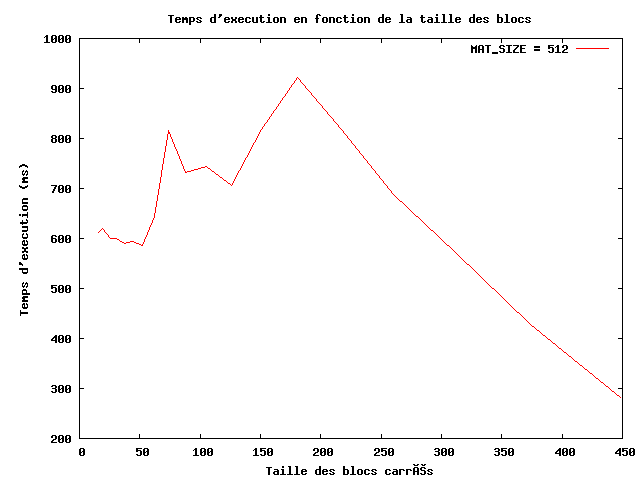
\includegraphics[width=\textwidth]{data_dgetrf_2.png}
\caption{2 processus}
\label{fig:d_2}
\end{subfigure}
\begin{subfigure}[b]{0.48\textwidth}
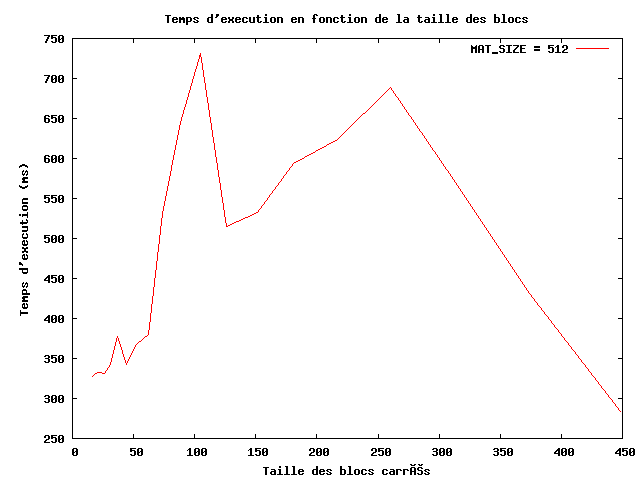
\includegraphics[width=\textwidth]{data_dgetrf_4.png}
\caption{4 processus}
\label{fig:d_4}
\end{subfigure}

\begin{subfigure}[b]{0.48\textwidth}
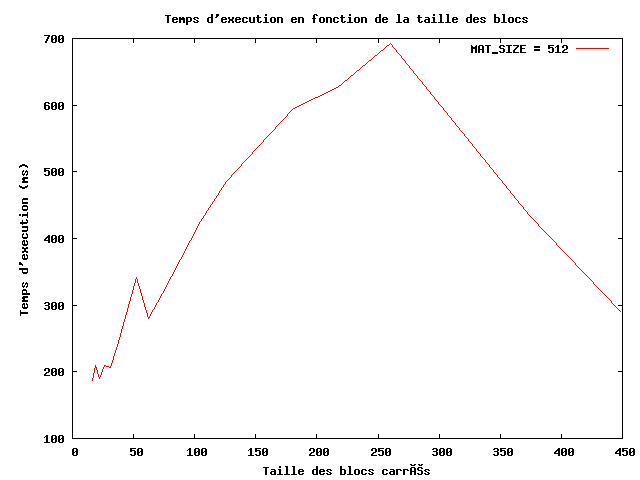
\includegraphics[width=\textwidth]{data_dgetrf_8.png}
\caption{8 processus}
\label{fig:d_8}
\end{subfigure}
\begin{subfigure}[b]{0.48\textwidth}
\centering
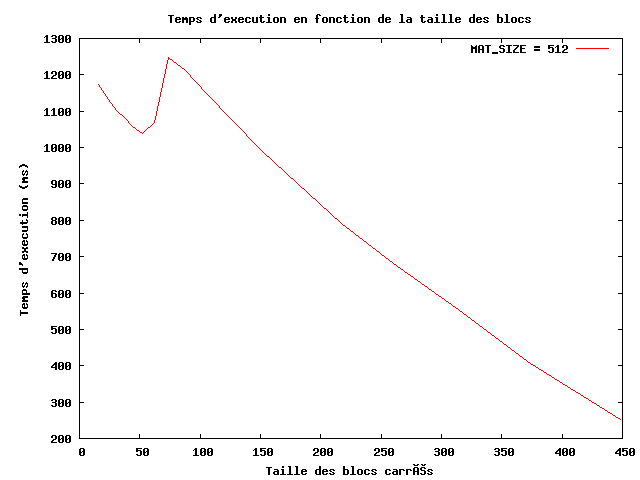
\includegraphics[width=\textwidth]{data_dgetrf_seq.png}
\caption{version séquentielle}
\label{fig:d_s}
\end{subfigure}
\caption{Temps d'exécution en fonction de la taille des blocs, pour un nombre différent de processus.}
\end{figure}


\section*{Conclusion}
\addcontentsline{toc}{section}{Conclusion}

Ce TDP nous a fait travailler en profondeur les fonctions classiques de calcul matriciel. Malheureusement nous n'avons pas été jusqu'au bout en introduisant les mécanismes de pivotage dans notre implémentation de la factorisation LU, ni le calcul parallèle dans la résolution d'un système linéaire triangulaire. Nous regrettons de plus les résultats que nous avons obtenus, qui ne correspondent pas à nos attentes.


\end{document}
